% Talk accompanying docs/report. Seventeen slides for about fifteen minutes,
% plus backup. Built with pdfLaTeX, like the report. The spoken part of each
% slide is in \note{}: compile as is for the deck, or uncomment the line below
% to get the notes alongside it.
%
% \setbeameroption{show notes on second screen=right}

\documentclass[aspectratio=169,11pt]{beamer}

% The stock theme and colours, so the deck builds anywhere without a package
% beyond a plain TeX installation.
\usetheme{default}
\setbeamertemplate{navigation symbols}{}
\setbeamertemplate{itemize items}[circle]
\setbeamertemplate{caption}{\insertcaption}
\setbeamerfont{frametitle}{size=\large}
\setbeamertemplate{footline}{%
  \hfill\usebeamerfont{footline}\color{gray}\scriptsize
  \insertframenumber\,/\,\inserttotalframenumber\hspace{2ex}\vspace{1ex}%
}

\usepackage[T1]{fontenc}
\usepackage[english]{babel}
\usepackage{amsmath, amssymb}
\usepackage{graphicx}
\usepackage{booktabs}

\graphicspath{{assets/}{../report/assets/}{../figures/}{../../results/figures/}}

\title{Compressed Sensing using Generative Models}
\subtitle{Reproducing Bora, Jalal, Price \& Dimakis (ICML 2017)}
\author{Matteo Forlivesi \and Renato Gallicola}
\institute{Politecnico di Milano \\ Numerical Analysis for Machine Learning}
\date{}

\begin{document}

\begin{frame}[plain]
  \titlepage
\end{frame}

% ---------------------------------------------------------------- 2
\begin{frame}{The problem}
  \begin{block}{}
    \[
      y = A x^{\ast} + \eta, \qquad
      A \in \mathbb{R}^{m \times n}, \qquad m \ll n
    \]
  \end{block}
  \vspace{1em}
  \begin{center}
    \large Recover a 784 pixel image from 75 numbers.
  \end{center}
  \note{The system is underdetermined, so it has infinitely many solutions and
    recovery is impossible without an assumption about which solutions are
    plausible. Everything that follows is about what that assumption should be.}
\end{frame}

% ---------------------------------------------------------------- 3
\begin{frame}{The classical assumption: sparsity}
  \[
    \hat\theta = \arg\min_\theta \lVert A \Psi \theta - y \rVert_2^2
      + \alpha \lVert \theta \rVert_1,
    \qquad \hat x = \Psi \hat\theta
  \]
  \begin{center}
    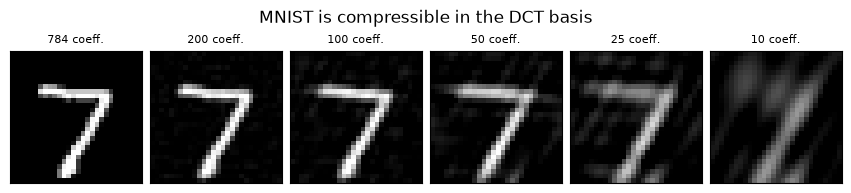
\includegraphics[width=0.95\linewidth]{dct_truncation}
  \end{center}
  \note{MNIST really is compressible in the DCT basis: 25 coefficients out of
    784 still give a recognisable digit. But compressed sensing does not get to
    choose which coefficients to keep, it has to discover their support from
    random projections, and that is what costs measurements.}
\end{frame}

% ---------------------------------------------------------------- 4
\begin{frame}{The idea: replace sparsity with a learned prior}
  \begin{columns}[T]
    \begin{column}{0.48\textwidth}
      \begin{center}
        \textbf{Sparsity} \\[0.6em]
        ``few non-zero coefficients''
      \end{center}
    \end{column}
    \begin{column}{0.48\textwidth}
      \begin{center}
        \textbf{Generative prior} \\[0.6em]
        ``looks like a digit''
      \end{center}
    \end{column}
  \end{columns}
  \vspace{1em}
  \begin{center}
    
\includegraphics[width=0.62\linewidth]{prior_samples}
  \end{center}
  \note{A trained generator maps a low dimensional latent vector to an image,
    and its range is the set of images it can produce. These samples are the
    entire hypothesis space of the method, which will matter on slide 12.}
\end{frame}

% ---------------------------------------------------------------- 5
\begin{frame}{The three priors}
  \begin{center}
    \begin{tabular}{lll}
      \toprule
      & trained by & architecture \\
      \midrule
      VAE        & maximising the ELBO       & convolutional, ours \\
      DCGAN      & adversarial minimax game  & convolutional, ours \\
      VAE, paper & maximising the ELBO       & fully connected 784-500-500-20 \\
      \bottomrule
    \end{tabular}
  \end{center}
  \vspace{1em}
  Baselines: LASSO in the pixel basis, which is what the paper uses on MNIST,
  and LASSO in the DCT basis.
  \note{The first two are our own designs, each trained at latent dimension 20
    and 30. The third is the network Bora et al. actually use on MNIST. We
    included it because our own models are not theirs, so without it a gap
    between our numbers and theirs could be blamed either on the method or on
    the model, and we could not tell which. Worth saying explicitly: the paper
    never runs a GAN on MNIST, so that half of the comparison is our own
    extension.}
\end{frame}

% ---------------------------------------------------------------- 6
\begin{frame}{Recovery}
  \[
    \hat z = \arg\min_z \lVert A G(z) - y \rVert_2^2
      + \lambda \lVert z \rVert_2^2,
    \qquad \hat x = G(\hat z)
  \]
  \begin{center}
    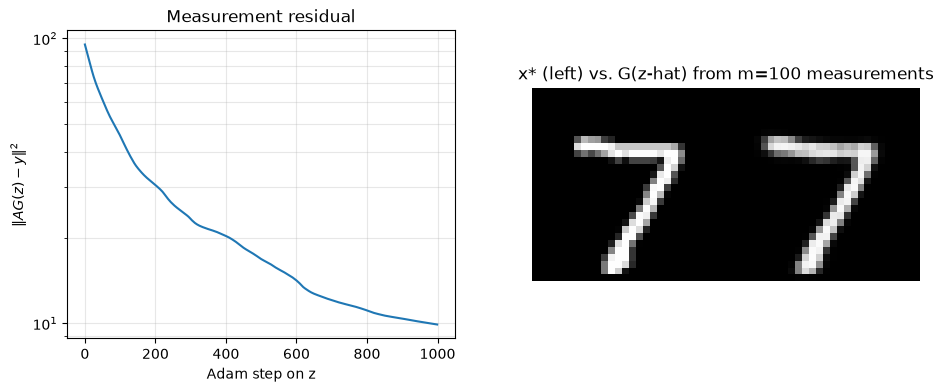
\includegraphics[width=0.82\linewidth]{recovery_residual}
  \end{center}
  \note{Gradient descent on the latent vector, not on the weights: the generator
    is frozen and the only variable is twenty or thirty numbers. The second term
    is the prior: since z is Gaussian under both models, its squared norm is the
    negative log-likelihood. Point at the residual falling by orders of
    magnitude and then flattening, and say that what remains is not an
    optimisation failure. This sets up slide 12.}
\end{frame}

% ---------------------------------------------------------------- 7
\begin{frame}{The objective is not convex}
  \begin{center}
    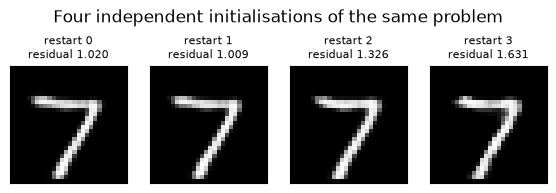
\includegraphics[width=0.8\linewidth]{restarts}
  \end{center}
  \note{G is a deep network, so different initialisations reach different local
    minima. We run ten restarts and keep the smallest measurement error. Note
    two things: the measurement error is computable from y alone, without the
    ground truth, so the rule is legitimate; and the penalty is deliberately
    excluded from it, since ranking on the full objective would reward a small
    latent norm rather than a good reconstruction.}
\end{frame}

% ---------------------------------------------------------------- 8
\begin{frame}{Why so few measurements are enough}
  \begin{block}{}
    If \( G \) is \( L \)-Lipschitz, of the order of \( k \log L \) random
    Gaussian measurements suffice to come within a constant of the best
    reconstruction available in the range of \( G \).
  \end{block}
  \note{The cost scales with the latent dimension k, not the ambient dimension
    n. 784 pixels but only 20 or 30 degrees of freedom, so the measurement
    budget is driven by 20 or 30.}
\end{frame}

% ---------------------------------------------------------------- 9
\begin{frame}{Experimental protocol}
  \begin{itemize}
    \item Ten test digits, one per class.
    \item The same measurement matrix and the same noise for every method at
      every budget.
    \item Noise with a fixed expected norm of 0.1, so budgets stay comparable.
    \item Error is the squared distance to the ground truth, per pixel.
  \end{itemize}
  \note{Insist on the last point. The quantity plotted is the error against the
    true image, not the measurement error the optimiser minimises. The latter
    falls as m falls, simply because there are fewer constraints, so it says how
    well the optimisation converged and not how good the answer is.}
\end{frame}

% ---------------------------------------------------------------- 10
\begin{frame}{Results}
  \begin{center}
    
\includegraphics[width=0.86\linewidth]{error_vs_measurements}
  \end{center}
  \note{At 25 measurements the best prior reaches 0.0194 against 0.0986 for the
    DCT baseline, 5.1 times better, at a budget where neither baseline returns
    anything recognisable. Either baseline needs 400 measurements to reach about
    0.011; all three VAE priors get there with 75, a 5.3x saving, and the factor
    is the same against both baselines. The paper reports 5 to 10x, so we land
    at the bottom of that range. The DCGAN at k=30 needs 300, a 1.3x saving; the
    one at k=20 never gets there. If asked about the pixel baseline: predicting
    a blank image scores 0.1178 on these digits, and the pixel baseline is at or
    above that at 10 and 25 measurements, so a ratio against it there compares
    against nothing.}
\end{frame}

% ---------------------------------------------------------------- 11
\begin{frame}{What the reconstructions look like}
  \begin{center}
    
\includegraphics[width=0.92\linewidth]{reconstruction_grid}
  \end{center}
  \note{The DCT baseline returns a noisy image until about 300 measurements and
    the pixel one an almost blank image until about 400, while every generative
    prior produces a plausible digit almost immediately. The DCGAN gives visibly
    sharper strokes, because an adversarial generator is pushed towards samples
    a discriminator accepts rather than towards the average of the plausible
    ones. But sharper is not more accurate: a crisp digit of the wrong shape
    scores worse than a slightly soft one of the right shape, and the table
    bears that out.}
\end{frame}

% ---------------------------------------------------------------- 12
\begin{frame}{The ceiling}
  \begin{center}
    \begin{tabular}{lc}
      \toprule
      prior & error floor \\
      \midrule
      VAE \( k = 30 \)          & 0.0070 \\
      VAE, paper architecture   & 0.0072 \\
      VAE \( k = 20 \)          & 0.0076 \\
      DCGAN \( k = 30 \)        & 0.0093 \\
      DCGAN \( k = 20 \)        & 0.0119 \\
      \bottomrule
    \end{tabular}
  \end{center}
  \vspace{0.5em}
  \begin{center}
    \small Averaged from 300 measurements up.
  \end{center}
  \note{Past roughly 200 measurements the learned priors stop improving. The
    bottleneck is no longer information, it is that the true digit is not in the
    range of G, and that distance does not depend on the budget. From 500
    measurements both baselines overtake everything, and at 750 the pixel one
    recovers the digits almost exactly while the priors stay put. The paper says
    the reversal takes more than 500 measurements; we see it from 500 onwards. A
    factor 1.7 separates the best floor from the worst, so on this side of the
    plot the generator still matters, though far less than the gap to the
    baselines does when measurements are scarce. If asked about the DCGANs: each
    was trained on the same 54,000 images as the VAEs, and the epoch used was
    chosen among seven saved candidates on held-out data, which earned about 11
    per cent in both runs. One seed each rather than the VAEs' two, because a
    run costs some fifteen hours.}
\end{frame}

% ---------------------------------------------------------------- 13
\begin{frame}{What survives the statistics}
  \begin{itemize}
    \item The three VAE priors cannot be told apart: every corrected p-value
      is 1.
    \item Every prior beats both baselines at 100 measurements and loses to both
      at 750.
    \item The VAE beats the DCGAN at \( k = 20 \) at nine budgets out of ten,
      and at \( k = 30 \) only while measurements are scarce.
  \end{itemize}
  \vspace{0.5em}
  \begin{center}
    \small Paired Wilcoxon signed-rank tests, Holm-corrected across the ten
    budgets within each pair of methods.
  \end{center}
  \note{Every method sees the same images and the same matrices, so the
    comparisons are paired and we test them that way. The three VAE floors span
    0.0005 and ten images cannot separate that; say this plainly and do not rank
    them from the table. The crossover is the reproduction and it is the claim
    that survives correction: be precise if pressed, 50, 75, 100 and 300 are the
    budgets where it holds for all five priors at once, because the two DCGAN
    columns drop out elsewhere, and each VAE on its own is significantly better
    from 25 to 300. Every VAE has the lower mean error than every DCGAN at every
    budget; against k=30 ten images are not enough to prove it beyond the low
    budgets. If asked whether the penalty is unfair to the GANs: we ran them at
    0.001 too, the value the paper gives for a DCGAN, and it does not help.
    Saying out loud which differences do not reach significance is worth more
    than claiming five results and defending three.}
\end{frame}

% ---------------------------------------------------------------- 14
\begin{frame}{The latent regulariser}
  \begin{center}
    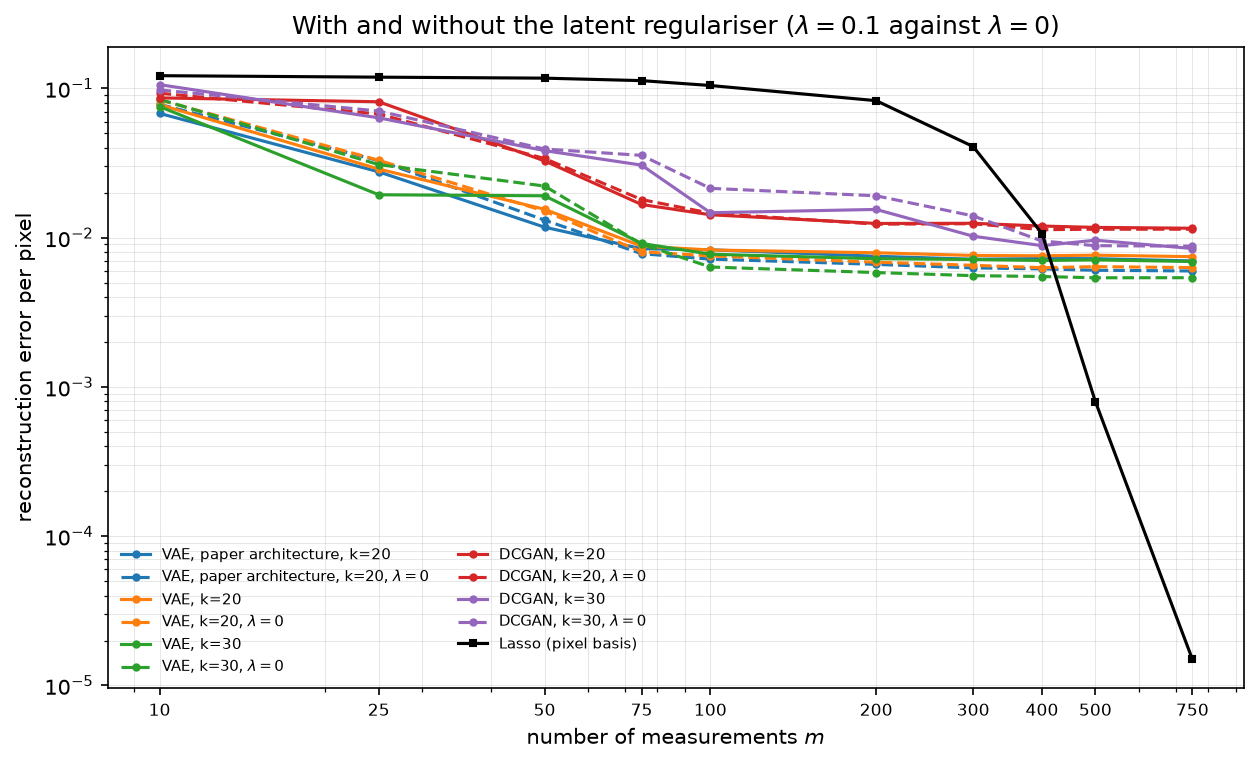
\includegraphics[width=0.86\linewidth]{regularisation_comparison}
  \end{center}
  \note{The paper uses lambda equal to 0.1 and plots both variants, so we did
    the same. It helps exactly where the measurements underdetermine the code:
    at 10 measurements it takes the best model from 0.0782 to 0.0680, a 13 per
    cent gain. It costs slightly once measurements are plentiful, 0.0054 to
    0.0069 at 750, because the same pull towards the prior keeps the solution
    off the closest point in the range. The sweep confirms the mechanism: the
    norm of the recovered code falls monotonically from 9.95 to 2.67, and the
    best value of lambda is not fixed but falls with the budget, 1 at 10
    measurements and 0 from 200 up. The single value the paper recommends is a
    compromise, not an optimum at any one budget. Note also that 0.1 is the
    value the paper gives for its MNIST VAE; for its DCGAN it gives 0.001, which
    we do not use, so the DCGAN columns carry a penalty that was never validated
    for them. This is the slide to drop if you are running short.}
\end{frame}

% ---------------------------------------------------------------- 15
\begin{frame}{Cost}
  \begin{center}
    \begin{tabular}{lc}
      \toprule
      method & seconds to recover 10 images at one budget \\
      \midrule
      LASSO, either basis      & about 1.5 \\
      VAE, paper architecture  & 6.6 \\
      VAE, convolutional       & 15 and 19 \\
      DCGAN                    & about 600 \\
      \bottomrule
    \end{tabular}
  \end{center}
  \note{A 93x gap between the cheapest and the dearest learned prior. Parameter
    count does not explain it: the DCGAN generator is only 4.5x larger, and our
    convolutional decoder is smaller than the paper's yet twice as slow. What it
    tracks is arithmetic per forward pass, and the DCGAN convolves 256 and 512
    channels at nearly full resolution. The cost is paid at every
    reconstruction, since recovery is itself an optimisation. And the punchline:
    the two most expensive priors are also the two least accurate, at every
    budget.}
\end{frame}

% ---------------------------------------------------------------- 16
\begin{frame}{A result about the method, not the models}
  \begin{center}
    \Large Training the same VAE with different random seeds gave generators
    whose quality varied by a factor of \textbf{3.5}.
  \end{center}
  \vspace{0.8em}
  \begin{center}
    Comparable to the entire spread between the architectures we set out to
    compare.
  \end{center}
  \note{The cause was partial posterior collapse: the decoder leaning on a
    handful of latent directions and ignoring the rest, which we measured
    directly. Adding a KL warm-up fixed it, and the spread across seeds is a
    factor of 2.5, 1.3 and 1.2 for the three configurations. That figure and the
    3.5 are measured on different images and over a different number of seeds,
    so do not present them as one ratio shrinking. The point to land: before
    this we would have reported that latent dimension 30 beats 20 by a wide
    margin, and that conclusion would have been an artefact of comparing a lucky
    run against an unlucky one. Any comparison between priors is only meaningful
    once it is larger than the variability of the procedure that produced them.
    The selection rules were written down before the runs, and are in the
    repository.}
\end{frame}

% ---------------------------------------------------------------- 17
\begin{frame}{Conclusions}
  \begin{itemize}
    \item A learned prior is worth about five times fewer measurements where
      measurements are scarce, which is the regime compressed sensing exists
      for, and that reproduces the reference paper.
    \item It buys that with a ceiling set by the generator, and with a
      reconstruction orders of magnitude more expensive.
    \item The three VAE generators could not be told apart with ten test images,
      so the training run mattered more than the architecture.
  \end{itemize}
  \note{Close on where this matters. Medical imaging, and any setting where a
    single measurement is slow, expensive or harmful to the subject, and where
    the reconstruction is done once.}
\end{frame}

% ================================================================ backup
\appendix

\begin{frame}[plain]
  \begin{center}
    \Large Backup
  \end{center}
\end{frame}

\begin{frame}{LASSO reconstructions across budgets}
  \begin{center}
    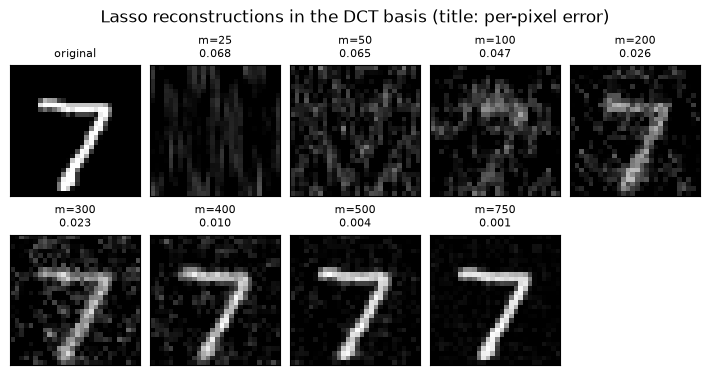
\includegraphics[width=0.92\linewidth]{lasso_reconstructions}
  \end{center}
\end{frame}

\begin{frame}{The two dimensional VAE latent space}
  \begin{center}
    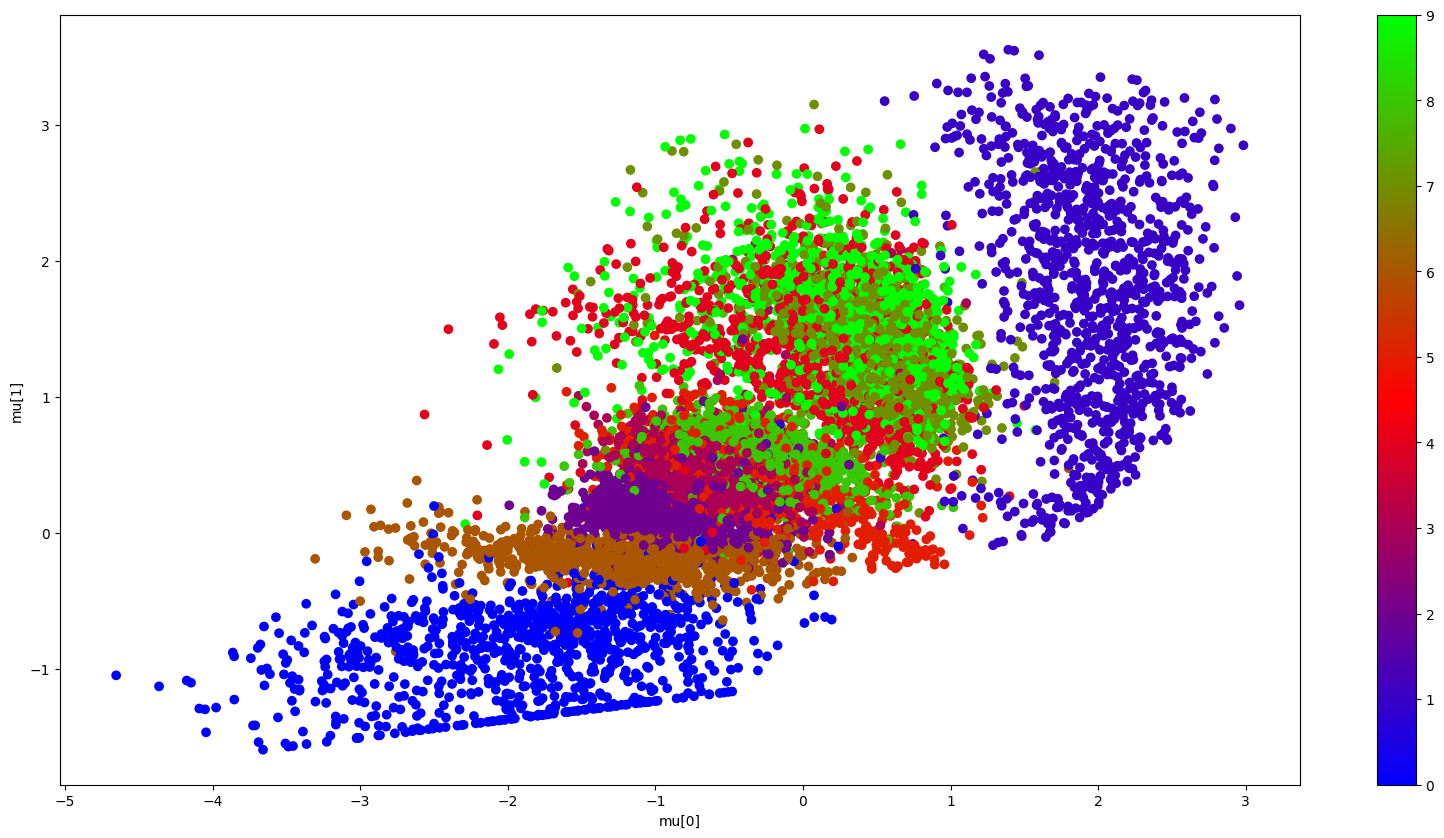
\includegraphics[width=0.55\linewidth]{vae_latent_space_2d}
  \end{center}
\end{frame}

\begin{frame}{ELBO components during VAE training}
  \begin{center}
    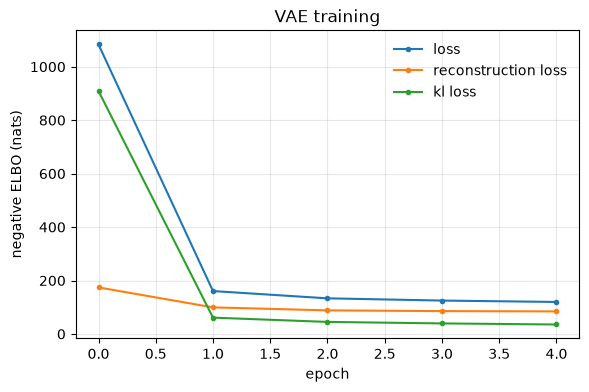
\includegraphics[width=0.8\linewidth]{vae_training}
  \end{center}
\end{frame}

\begin{frame}{How hard the GAN was to train}
  \begin{columns}[T]
    \begin{column}{0.48\textwidth}
      \begin{center}
        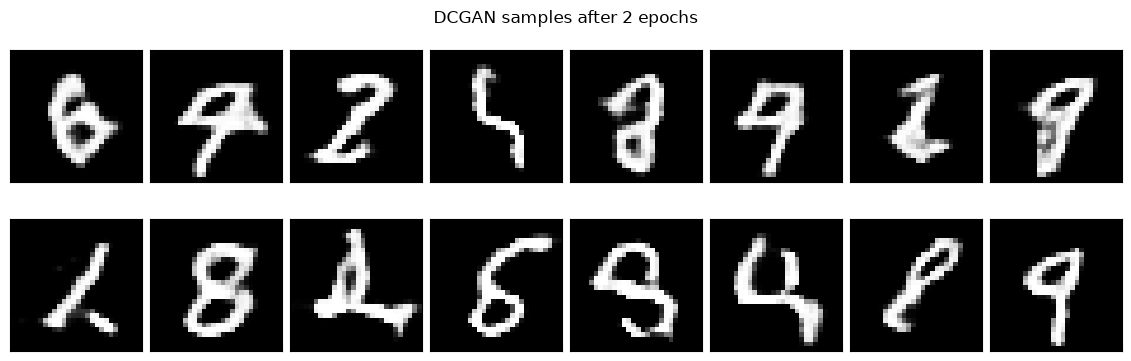
\includegraphics[width=\linewidth]{dcgan_early} \\
        \small after two epochs
      \end{center}
    \end{column}
    \begin{column}{0.48\textwidth}
      \begin{center}
        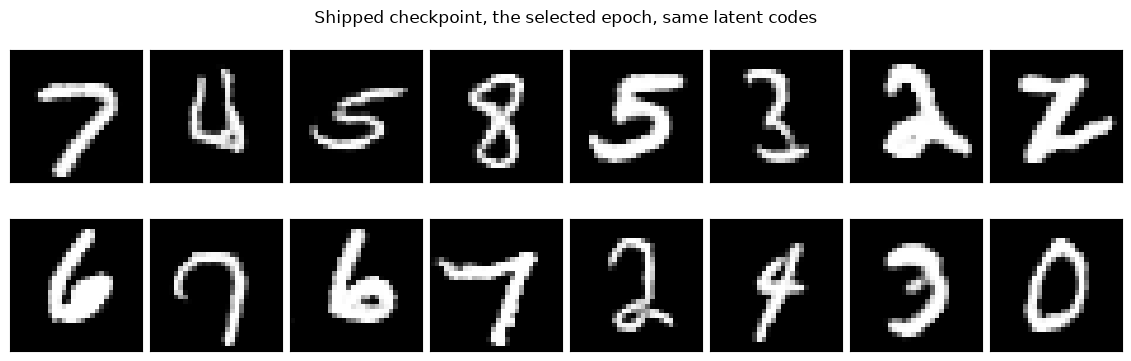
\includegraphics[width=\linewidth]{dcgan_selected} \\
        \small the selected checkpoint
      \end{center}
    \end{column}
  \end{columns}
\end{frame}

\begin{frame}{The full sweep over the regulariser}
  \begin{center}
    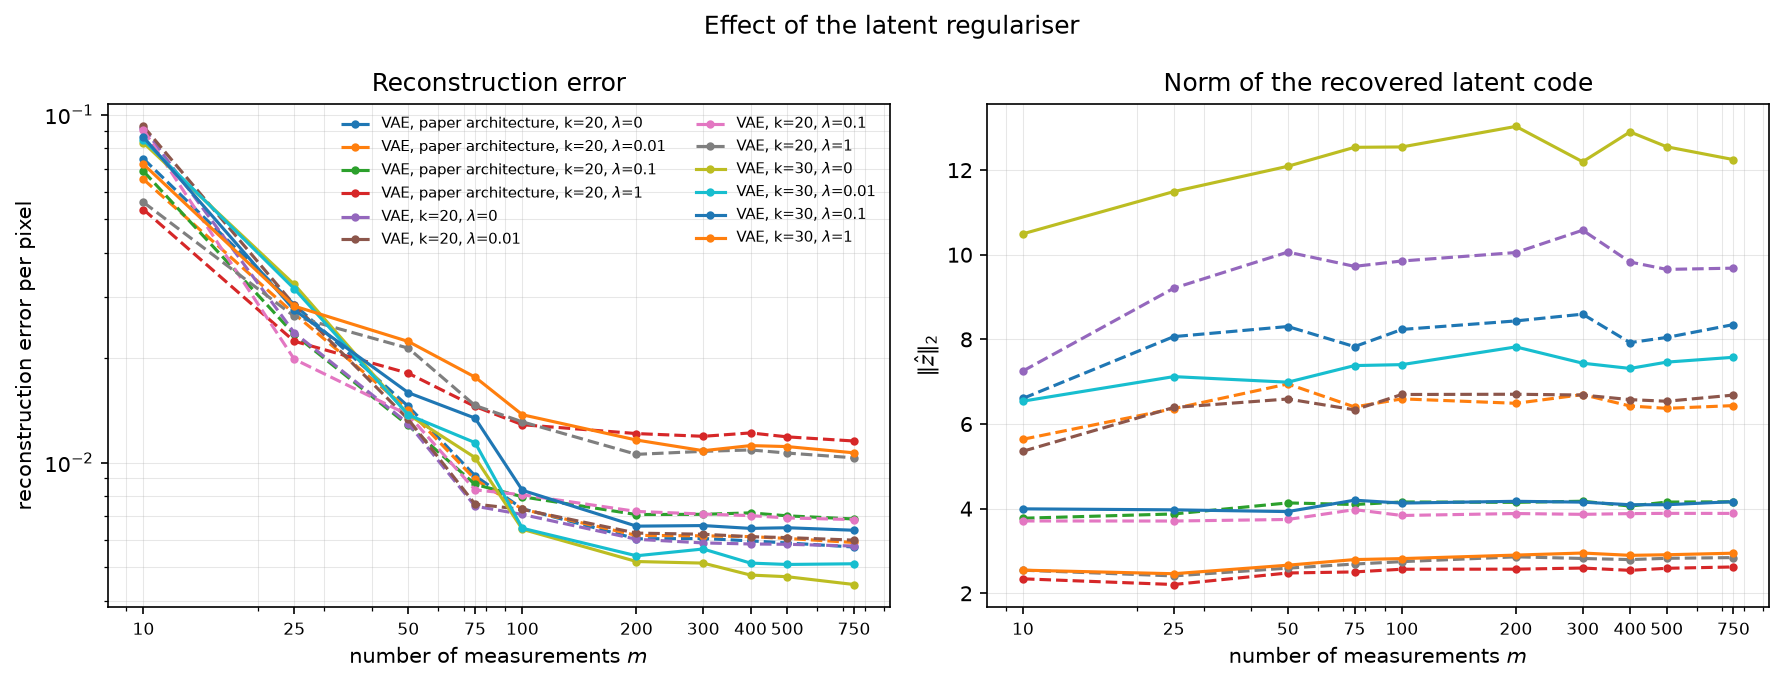
\includegraphics[width=0.86\linewidth]{lambda_sweep}
  \end{center}
\end{frame}

\end{document}
